\UseRawInputEncoding
\documentclass[12pt]{article}
\title{ECE 102 Project}
\usepackage{subcaption}
\author{Lawrence Liu}
\usepackage{graphicx}
\usepackage{amsmath}
\usepackage[scr]{rsfso}
\usepackage{placeins}
\newcommand{\Laplace}{\mathscr{L}}
\setlength{\parskip}{\baselineskip}%
\setlength{\parindent}{0pt}%
\usepackage{xcolor}
\usepackage{listings}
\definecolor{backcolour}{rgb}{0.95,0.95,0.92}
\usepackage{amssymb}
\lstdefinestyle{mystyle}{
    backgroundcolor=\color{backcolour}}
\lstset{style=mystyle}

\begin{document}
\maketitle
\section{Part I}
\subsection*{Step 1}
\subsubsection*{(a)}
We have $$\left(X(s)-kY(s)\right)H_1(s) H_2(s)=Y(s)$$
$$X(s)H_1(s) H_2(s)=Y(s)\left(1+k H_1(s) H_2(s)\right)$$
$$H(s)=\frac{Y(s)}{X(s)}=\boxed{\frac{H_1(s) H_2(s)}{1+k H_1(s) H_2(s)}}$$
\subsubsection*{(b)}
We have
$$Z(s)=(s-1)X(s)$$
$$H_1(s)=\boxed{(s-1)}$$
And we have
$$y(t)=\int_{-\infty}^{t} z(\tau)e^{4(\tau -t)}d\tau$$
$$y(t)=z(t)*e^{-4t}u(t)$$
$$Y(s)=Z(s)\frac{1}{s+4}$$
$$H_2(s)=\boxed{\frac{1}{s+4}}$$
\subsubsection*{(c)}
We have
$$H(s)=\frac{Y(s)}{X(s)}=\frac{H_1(s) H_2(s)}{1+k H_1(s) H_2(s)}$$
$$H(s)=\frac{s-1}{s+4+ks-k}$$
$$H(s)=\boxed{\frac{s-1}{(k+1)s+4-k}}$$
\subsubsection*{(d)}
The system has a pole at $$s=\frac{k-4}{k+1}$$
Therefore in order for this system to be stable we must have that the ROC covers $s=0$, ie that 
$$\frac{k-4}{k+1}<0$$
and thus
$$k-4<0$$
and 
$$k+1>0$$
thus we get
$$\boxed{-1\neq k<4}$$
\subsubsection*{(e)}
using this code, we get
\lstinputlisting[language=Matlab]{Step1Part1.m}
\begin{center}
\begin{figure}[h]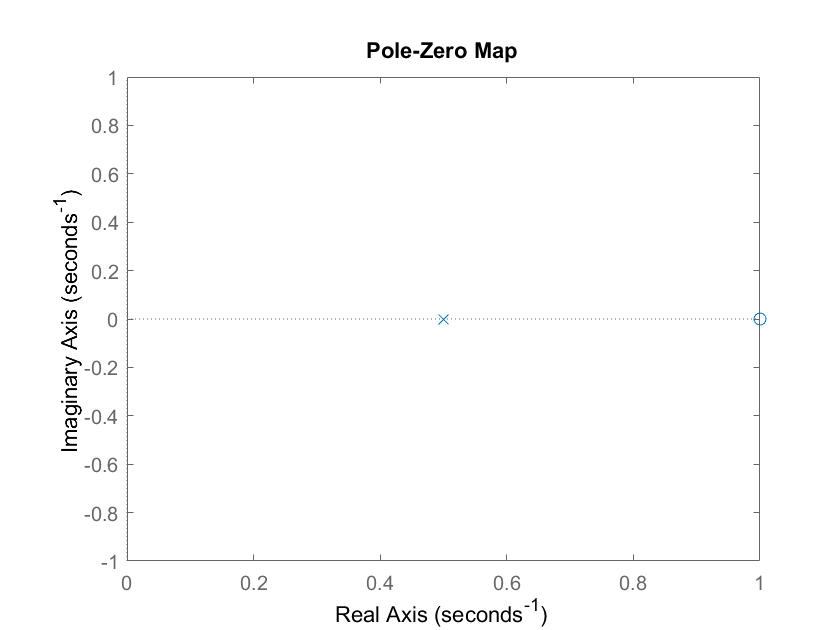
\includegraphics[width=8cm]{fig1}
\end{figure}
This plot, with $K=K_1=-3$ is unstable since there is a pole greater than $0$. But by changing $K$ to be $K=K_2=2$ the systems is stable since there are no poles greater than 0, the pole zero plot is included below. 
\end{center}
\lstinputlisting[language=Matlab]{Step1Part2.m}
\begin{center}
\begin{figure}[h]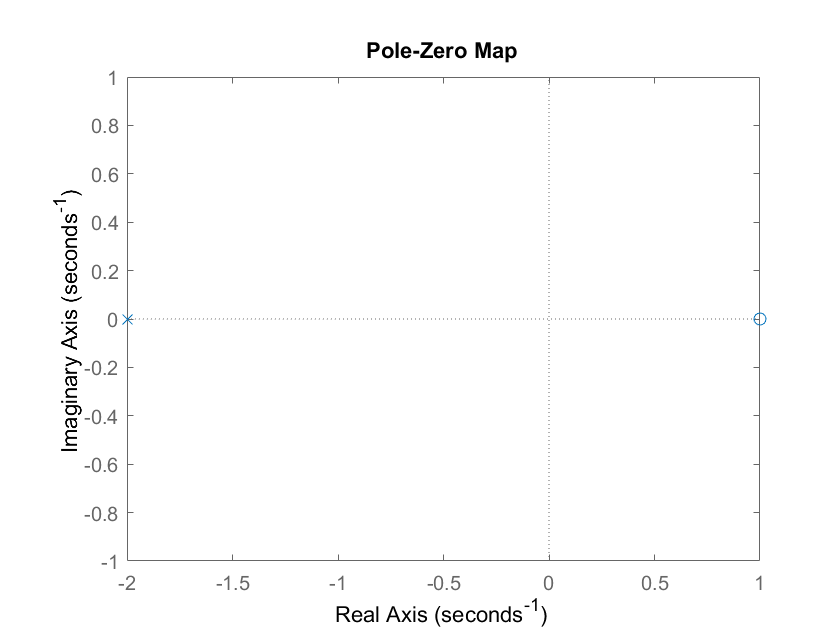
\includegraphics[width=8cm]{fig2}
\end{figure}
\end{center}
\subsection*{Step 2}
\subsubsection*{(a)}
\lstinputlisting[language=Matlab]{Step2Part1.m}
\begin{center}
\begin{figure}[h]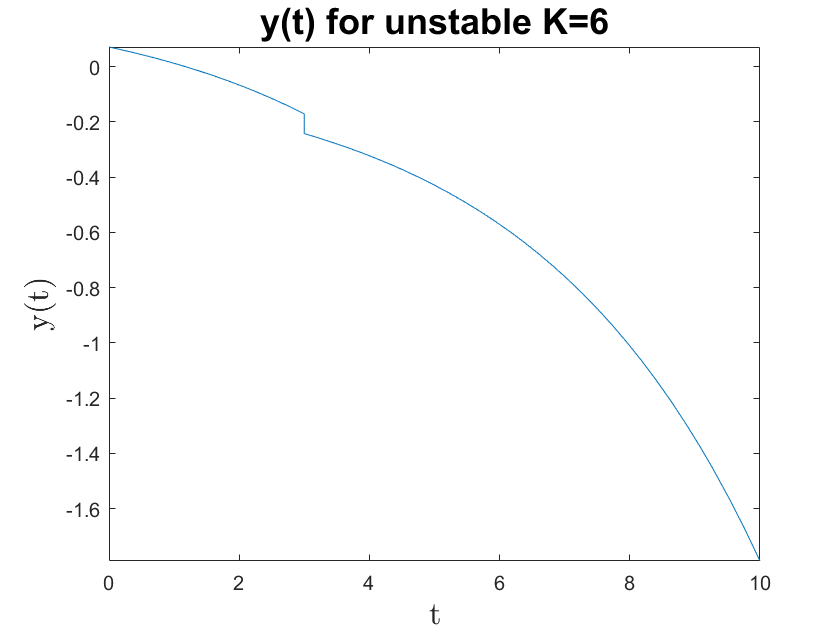
\includegraphics[width=8cm]{fig4}
\end{figure}
\end{center}
\FloatBarrier
And by changing the $K$ we get the following response for stable system
\begin{center}
\begin{figure}[h]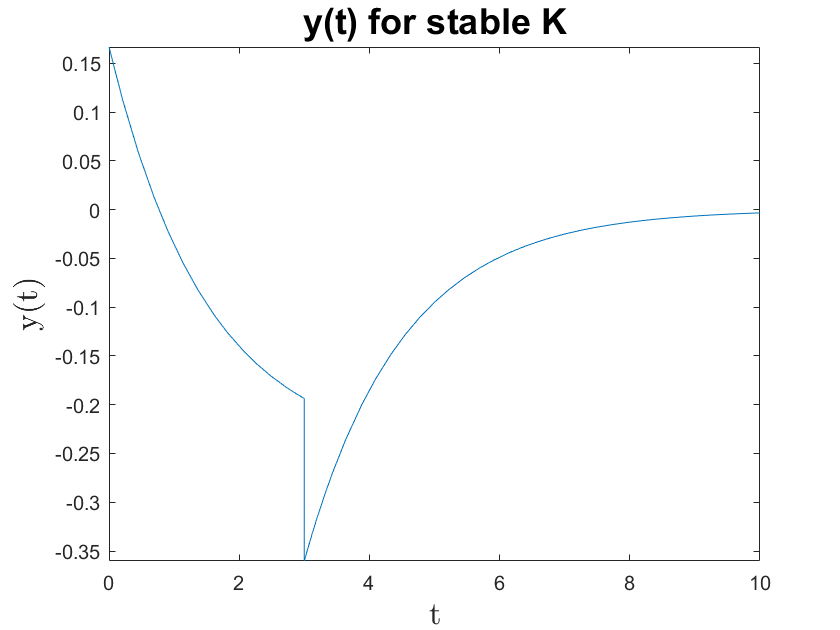
\includegraphics[width=8cm]{fig3}
\end{figure}
\end{center}
\FloatBarrier
\subsubsection*{(b)}
\lstinputlisting[language=Matlab]{Step2Part2.m}
\begin{center}
\begin{center}
\begin{figure}[h]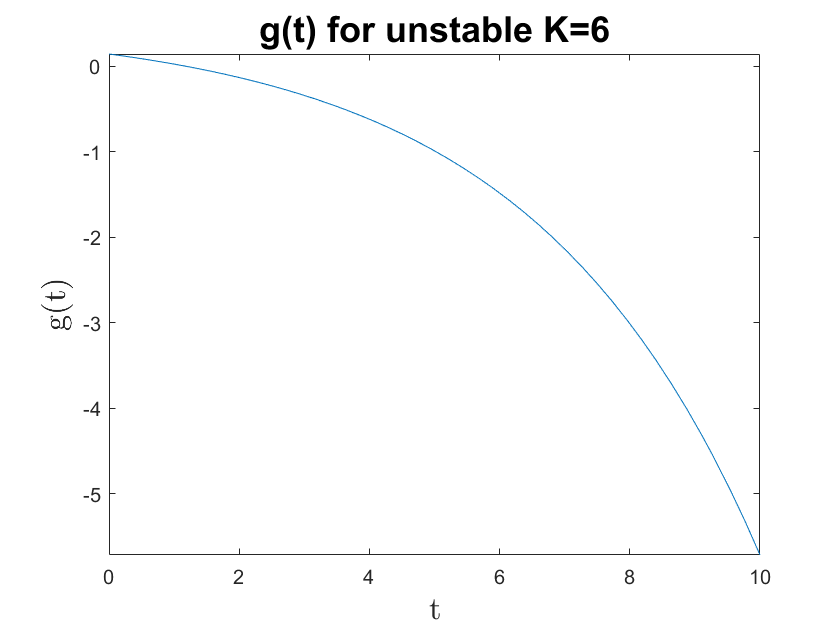
\includegraphics[width=8cm]{fig6}
\end{figure}
\end{center}
\FloatBarrier
And by changing the $K$ we get the following response for stable system
\begin{figure}[h]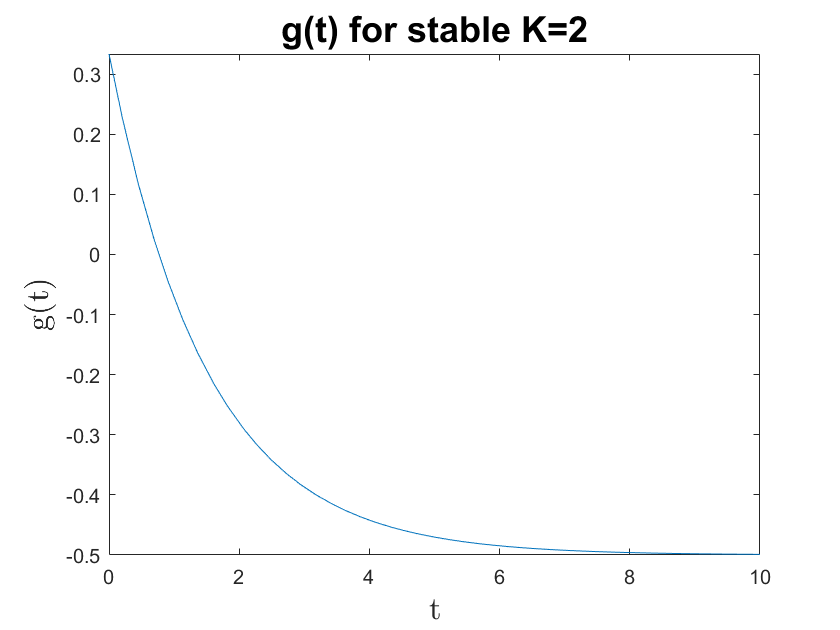
\includegraphics[width=8cm]{fig5}
\end{figure}
\end{center}
\FloatBarrier
\section*{Part 2}
\subsection*{Step 3}
\subsubsection*{(a)}
When $K=2$ we have
$$H(s)=\frac{s-1}{3s+2}$$
$$H(j\omega)=\boxed{\frac{j\omega-1}{3j\omega+2}}$$
\subsubsection*{(b)}
\lstinputlisting[language=Matlab]{Step3Part1.m}
\begin{center}
\begin{figure}[h]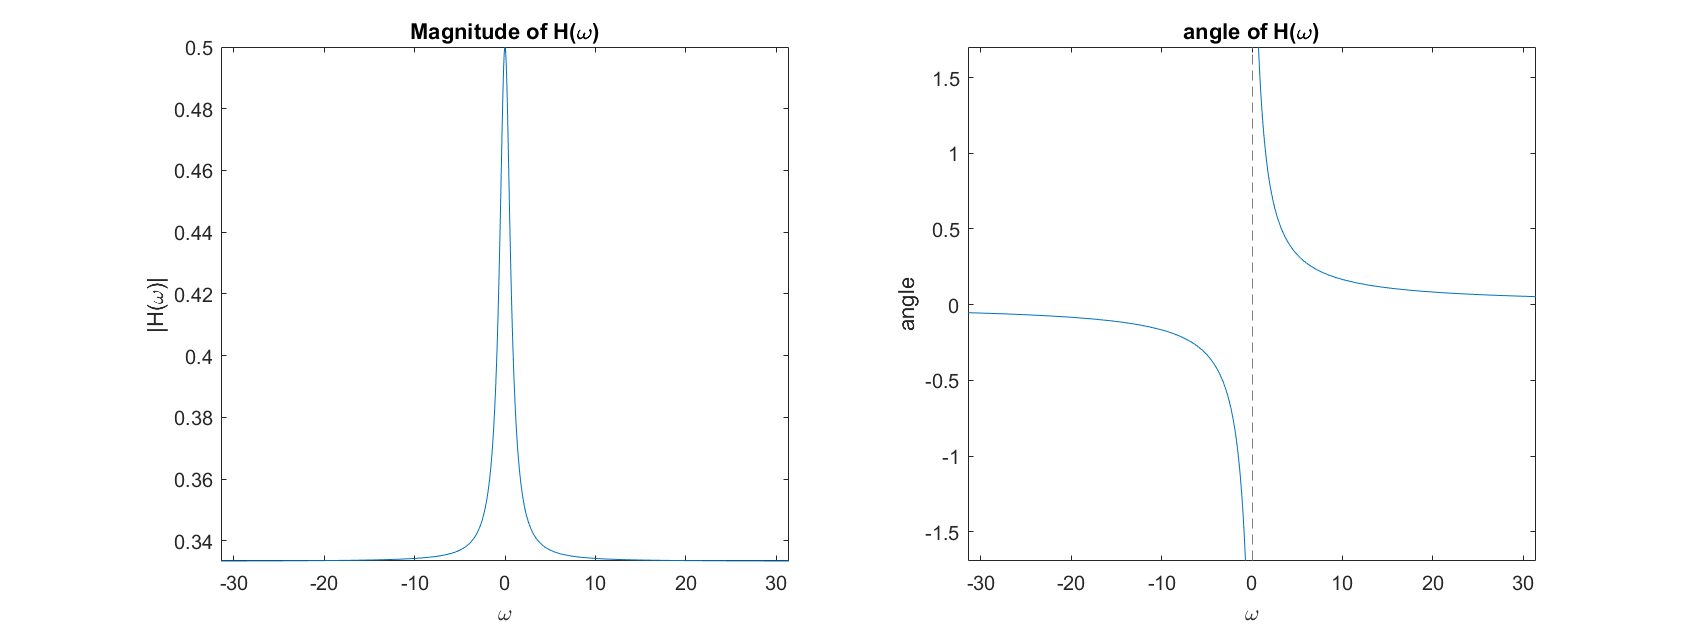
\includegraphics[width=15cm]{fig7}
\end{figure}
\end{center}
\FloatBarrier
\subsubsection*{(c)}
High frequency inputs are more heavily attenuated compared with low frequency inputs.
\subsection*{Step 4}
\subsubsection*{(a)}
\begin{align*}
a_k&=\frac{1}{4}\left(\int_{0}^{2}\frac{t}{2}e^{-jk\frac{\pi}{2}t}dt+\int_{2}^{4}e^{-jk\frac{\pi}{2}t}dt\right)\\
&=\frac{1}{4}\left(\dfrac{2\left(\left(\mathrm{j}{\pi}k+1\right)\cos\left({\pi}k\right)-1\right)}{{\pi}^2k^2}+\dfrac{2\left(\mathrm{j}\cos\left(2{\pi}k\right)-\mathrm{j}\cos\left({\pi}k\right)\right)}{{\pi}k}\right)\\
&=\boxed{\frac{1}{2}\left(\dfrac{\left(\left(\mathrm{j}{\pi}k+1\right)(-1)^k-1\right)}{{\pi}^2k^2}+\dfrac{\left(\mathrm{j}-\mathrm{j}(-1)^k\right)}{{\pi}k}\right)}
\end{align*}
\subsubsection*{(b)}
\lstinputlisting[language=Matlab]{Step4Part1.m}
\begin{center}
\begin{figure}[h]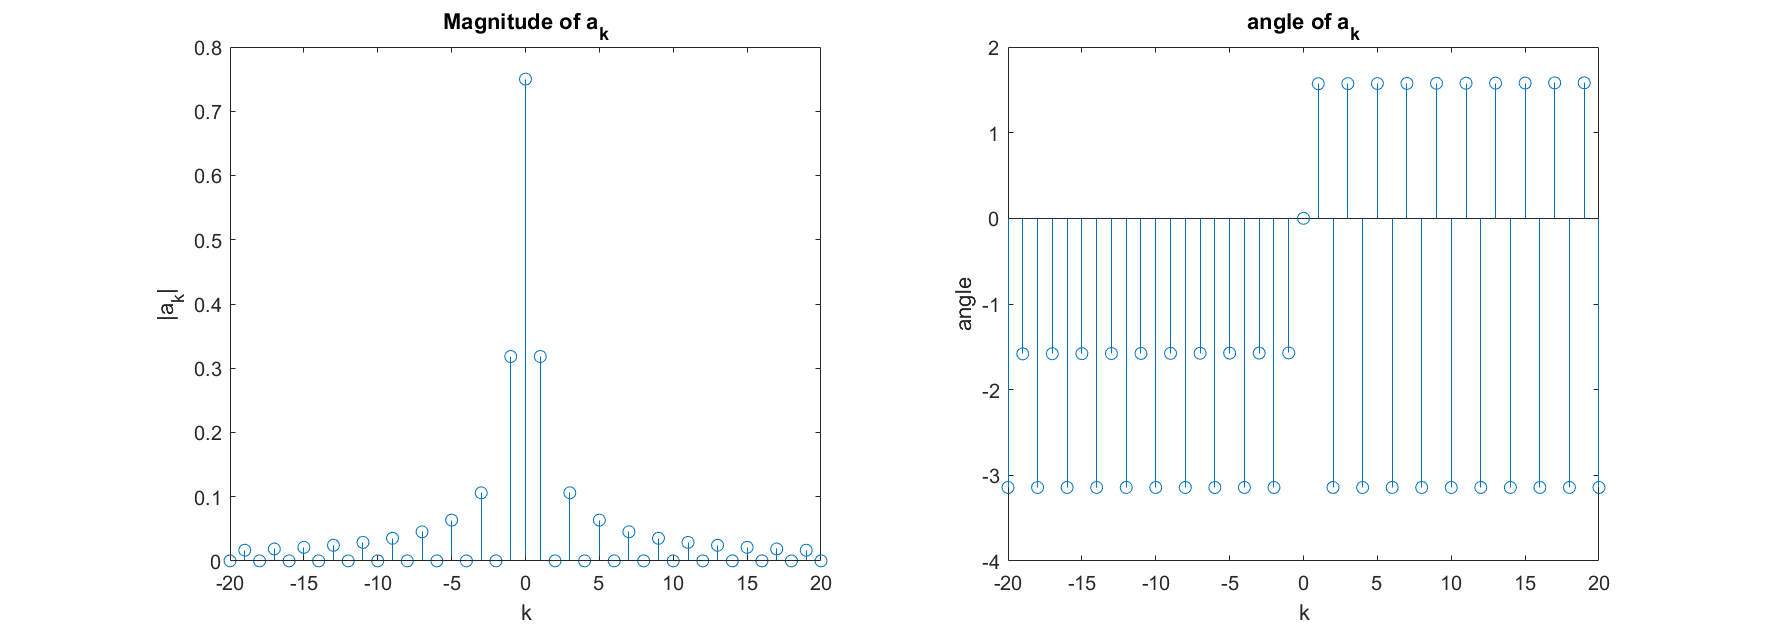
\includegraphics[width=15cm]{fig8}
\end{figure}
\end{center}
\FloatBarrier
\subsubsection*{(c)}
\begin{align*}
Y_k&=H(jk\frac{\pi}{2})a_k\\
&=\boxed{\frac{jk\frac{\pi}{2}-1}{2(3jk\frac{\pi}{2}+2)}\left(\dfrac{\left(\left(\mathrm{j}{\pi}k+1\right)(-1)^k-1\right)}{{\pi}^2k^2}+\dfrac{\left(\mathrm{j}-\mathrm{j}(-1)^k\right)}{{\pi}k}\right)}
\end{align*}
\subsubsection*{(d)}
\lstinputlisting[language=Matlab]{Step4Part2.m}
\begin{center}
\begin{figure}[h]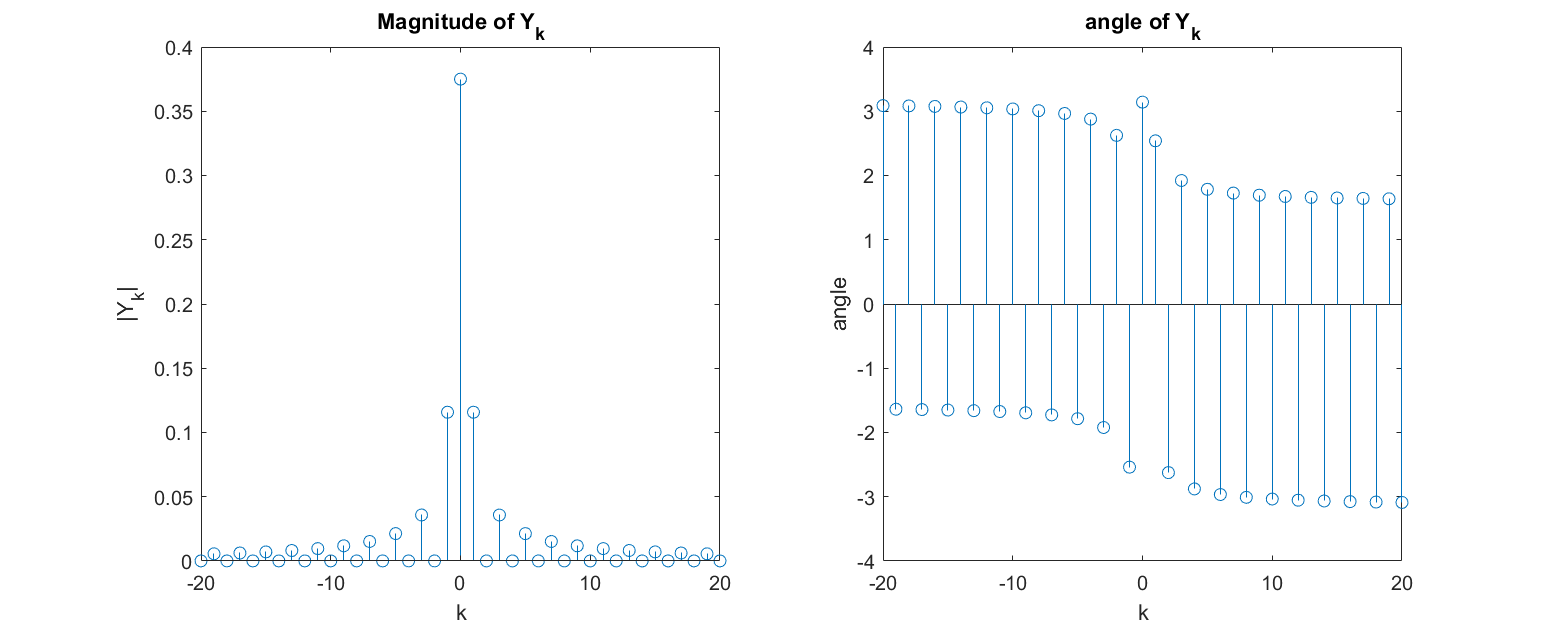
\includegraphics[width=15cm]{fig9}
\end{figure}
\end{center}
\FloatBarrier
\subsubsection*{(e)}
\lstinputlisting[language=Matlab]{Step4Part3.m}
\begin{center}
\begin{figure}[h]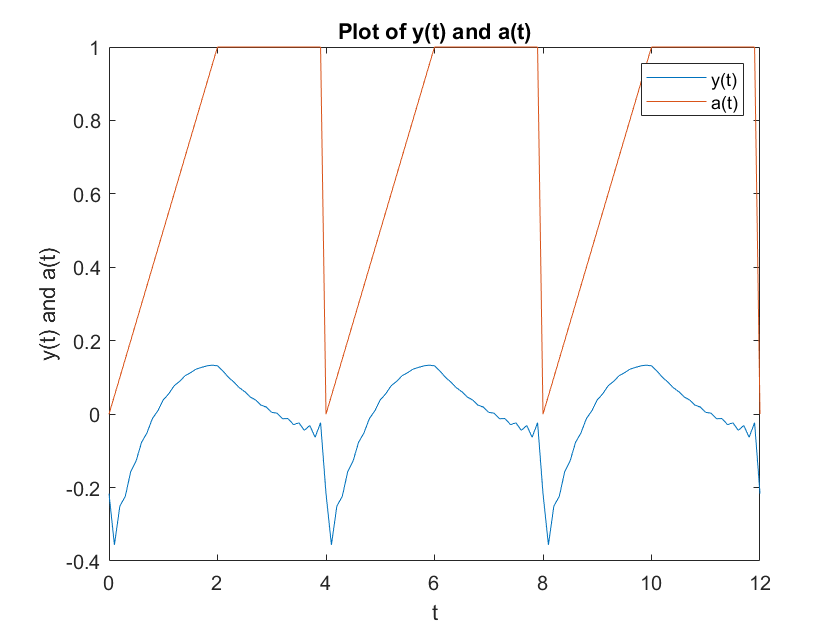
\includegraphics[width=10cm]{fig10}
\end{figure}
\end{center}
\FloatBarrier




\end{document}